\documentclass[10pt,twocolumn,letterpaper]{article}

\usepackage{iccv}
\usepackage{times}
\usepackage{epsfig}
\usepackage{graphicx}
\usepackage{amsmath}
\usepackage{amssymb}

% Include other packages here, before hyperref.

% If you comment hyperref and then uncomment it, you should delete
% egpaper.aux before re-running latex.  (Or just hit 'q' on the first latex
% run, let it finish, and you should be clear).
\usepackage[pagebackref=true,breaklinks=true,letterpaper=true,colorlinks,bookmarks=false]{hyperref}

% \iccvfinalcopy % *** Uncomment this line for the final submission

\def\iccvPaperID{****} % *** Enter the ICCV Paper ID here
\def\httilde{\mbox{\tt\raisebox{-.5ex}{\symbol{126}}}}

% Pages are numbered in submission mode, and unnumbered in camera-ready
\ificcvfinal\pagestyle{empty}\fi

\begin{document}

%%%%%%%%% TITLE
\title{CALVIS: Chest, wAist and peLVIS circumference from 3D human body meshes 
as ground truth for deep learning}

\author{Yansel González Tejeda\\
Paris Lodron University of Salzburg\\
{\tt\small yansel.gonzalez-tejeda@stud.sbg.ac.at}
% For a paper whose authors are all at the same institution,
% omit the following lines up until the closing ``}''.
% Additional authors and addresses can be added with ``\and'',
% just like the second author.
% To save space, use either the email address or home page, not both
\and
Helmut Mayer\\
{\tt\small helmut@cosy.sbg.ac.at}
}

\maketitle
% Remove page # from the first page of camera-ready.
\ificcvfinal\thispagestyle{empty}\fi

%%%%%%%%% ABSTRACT
\begin{abstract}
   In this paper we present CALVIS, a method to calculate chest, waist and 
   pelvis circumference from 3D human body meshes. Our motivation is to use 
   this data as ground truth for learning with convolutional neural networks 
   (CNN). Previous work had used the large scale CAESAR dataset, determined 
   $\textit{manually}$ these anthropometrical measurements or directly acquired 
   them from a person. The problem is that acquiring these data is a cost and 
   time consuming endeavor. In contrast our method can be used on 
   3D meshes automatically. First, we slice cross sections along the Y axis of 
   the mesh. Second, we calculate the cross sections length and establish a 
   signature for the body represented by the mesh. Finally, using this 
   signature we are able to calculate the chest, waist and pelvis 
   circumference by searching for critical points. We conduct two experiments. 
   In the first experiment we synthesize 10 human body meshes. Then we apply 
   CALVIS to calculate chest, waist and pelvis circumference. We evaluate the 
   results qualitatively. We observe that the measurements can indeed be used 
   to estimate the shape of a person. The second experiment serves as a 
   proof-of-concept where we use the calculated human dimensions as a ground 
   truth to train a small CNN. The idea is to establish the plausibility of our 
   approach. After having trained the network with our data, we demonstrate 
   that learning converges, achieving a 3 percent prediction error. 
   Furthermore, we make the implementation of CALVIS publicly available to 
   advance the field.
\end{abstract}

%%%%%%%%% BODY TEXT
\section{Introduction}

\textbf{Motivation} 
Predicting 3D human body measurements from images is crucial in several 
scenarios 
like virtual try-on, animating, ergonomics, computational forensics and 
even health and mortality estimation. Researches had 
named this 
measurements body intuitive controls (\cite{Allen.2003}), biometric 
measurements (\cite{Sigal.2008}), body dimensions 
(\cite{DBLP:conf/bmvc/ChenRC11}), semantical parameters (\cite{Yang.2014}), 
traditional anthropometric 
measurements 
(\cite{Wuhrer2011}) or only ``shape" as in human shape estimation 
(\cite{Guan.2013}, \cite{Bogo:ECCV:2016}, \cite{Loper.2015}, 
\cite{Dibra.2016a}, \cite{Pishchulin.2017}). In contrast, we assume a more 
anthropometric approach 
motivated by comprehensive compendiums like Panero and Zelnik, 1979 
\cite{panero1979human}.
Throughout this paper the term human body 
dimensions 
will be used to refer to the above measurements.

The problem of estimating human body dimensions  
having only an image is an under-constrained  (or inverse) problem. Information 
gets lost when a camera is 
used to capture the human body in 3D space to 'render' a 2D image.

To tackle this problem a supervised learning approach can be used. This approach
demands large amount of human body anthropometric measurements and is certainly 
one of the biggest challenges in the field.  Currently there 
is only one large-scale dataset, the Civilian American and 
European Surface Anthropometry Resource (CAESAR) \cite{robinette1999caesar} 
with 3D human body scans and their corresponding anthropometric measurements. 
This survey was extraordinarily large and resource intensive: around nine 
thousand people from Europe and the USA where scanned, it was conducted over 
more than five years and costed more than six million dollars.

In the past decade a noticeably amount of researchers have employed this 
dataset to investigate human shape estimation. Because the measurement 
acquiring process is resource intensive and requires large amount of human and 
material resources, this type of studies are rare and the data they offer is 
expensive. Therefore, it is important to explore alternative methods where 
human body measurements derived from real data can be obtained for 
investigation.

3D human body generative models offers such an alternative. We propose to 
synthesize 3D human body meshes using the SMPL \cite{Loper.2015} generative 
model. Once we have 
the 3D meshes we can compute chest, waist and pelvis circumference. The next 
step after obtaining the 
measurements is to use a camera model to render
images. Finally, in possession of this ground truth we can 
input this images to the learning algorithm and perform inference.

Explain method here in a very succinct way. balslfas iourgioafdnsva 
ihasoifghksv kiashdikhjioapgjgf oiasjojaspofdgjaposjg aisfhdgipoashfgihasghj 
aishgfiashgiahsfighaishg ihaspioghpaioshgpiasfgpi 
pjasoip09erujfdnaihg8qzßehgiqhfe.

Problem statement: given a 3D human body mesh $\mathcal{M}$ we look for a 
method capable to automatically output chest, waist and pelvis circumference.

%------------------------------------------------------------------------
\section{Approach}

In this work we synthesize 3D human meshes using the SMPL
model \cite{Loper.2015}. This model is at its top level a skinned articulated 
model, i.e., 
consists of a 
surface mesh that mimics the skin and a skeleton related to that mesh. It is 
defined by a mean 
template shape represented by a vector of $N$ concatenated vertices 
$\mathbf{\bar{T}}$ in the zero pose, $\vec{\theta}^*$. In order 
to 
synthesize a 
new human mesh one has to deform the provided template mesh by 
setting shape parameters $\vec{\beta}$ and pose parameters $\vec{\theta}$. The 
model provides learned parameters
\begin{equation} \label{eq:smpl_params}
\Phi = \{\mathbf{\bar{T}}, \mathcal{W}, \mathcal{S}, \mathcal{J}, 
\mathcal{P}\}
\end{equation}
As mentioned above $\mathbf{\bar{T}}$ is the mean template shape. The weight 
matrix $\mathcal{W}$ represents how much the rotation of skeleton parts affects 
the vertices. In addition, the matrices $\mathcal{S}$ and $\mathcal{P}$ define 
linear functions that are used to deform $\mathbf{\bar{T}}$ and the matrix 
$\mathcal{J}$ predicts skeleton rest joint locations from vertices in the rest 
pose. We held fix these parameters during the synthesis.

\subsection{Human Body Mesh Signature}
Let us consider a human body mesh $\mathcal{M}$. Our method requires that 
$\mathcal{M}$ is standing with arms raised 
parallel to the 
ground at shoulder height at a $90^\circ$ angle. In the line 
of previous work (\cite{Dibra.2016a}), we name this pose the zero (also 
normalized (rf)) pose $\vec{\theta}^*$. Additionally, we assume that the mesh 
has LSA orientation, e.g., x, y and z axis are positively directed from 
right-to-left, inferior-to-superior and posterior-to-anterior, respectively. If 
the mesh has another orientation we can always apply transformations to 
LSA-align it.

Intuitively, we would like to measure the chest circumference bellow the arms 
at the widest part of the torso and the waist circumference at the 
narrowest part after the chest but above the hips. Similarly, the hip 
circumference is measured often around the widest part of hips and buttocks. We 
can formalize this intuition by considering the cross-sectional length of the 
2D intersection curves (\cite{book.compu.topo}) along the y-axis. Moreover, we 
can 
use a plane $\boldsymbol{\pi}$ parallel to the floor to intersect the mesh. 
Since $\mathcal{M}$ is 
triangulated, the boundary of this 
intersection is a collection of segments $s_i$. Therefore, we can 
determine the boundary length by specifying a point along the y-axis $j$ as
\begin{align}
\mathcal{BL}(\mathcal{M}, \boldsymbol{\pi}, j) = \sum_{i = 
1}^{i = n}s_i
\end{align}

Note that for cross sections where $\boldsymbol{\pi}$ intersects the legs, two 
disconnected curves will appear. That is by no means a problem because they are 
still a collection of segment with non-zero length.

\begin{figure}[t]
	\begin{center}
		%\fbox{\rule{0pt}{2in} \rule{0.9\linewidth}{0pt}}
		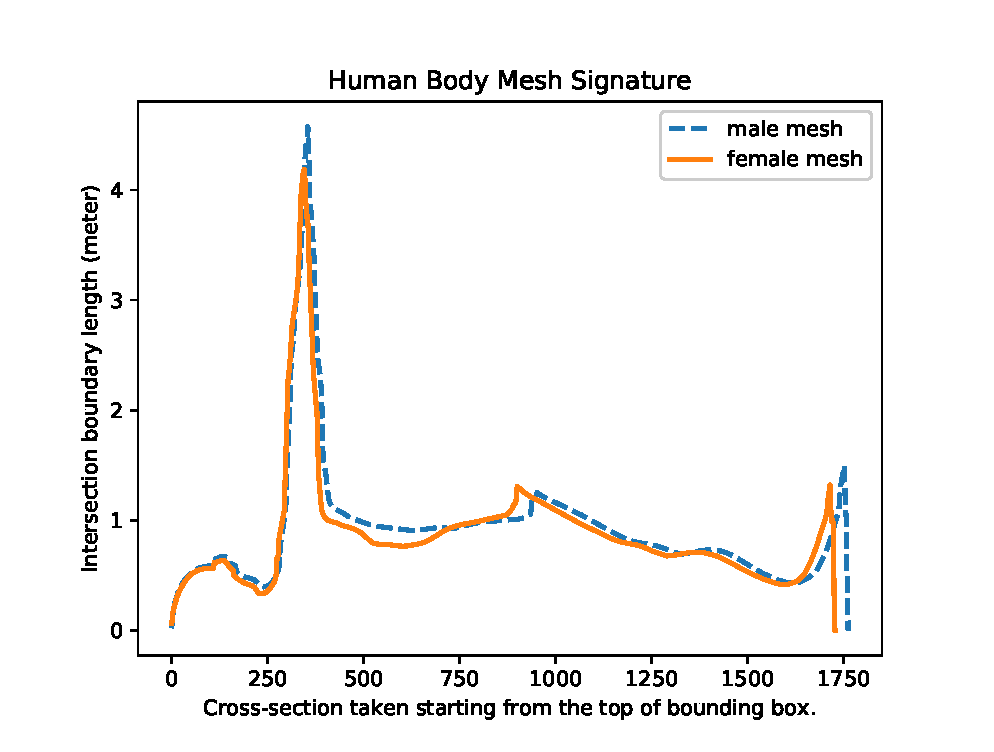
\includegraphics[width=\linewidth]{Figure_1.eps}
	\end{center}
	\caption{Human Body Mesh Signature for male and female meshes. The 
		function resembles a rotated silhouette of the human body and exhibits 
		several \textit{extrema}.}
	\label{fig:hbm_signature}
\end{figure}

Next, we assemble the mesh slide length vector $\vec{\mathcal{L}}$. Starting 
from the 
top $j_t$ of the bounding box we cut the mesh into 
evenly 
$m$-meters spaced slices until we reach the bounding box bottom $j_b$. For 
every 
slice at point $j$, we compute $\mathcal{BL}(j)$.

\begin{align}
\vec{\mathcal{L}} = \mathcal{BL}(j), \, j 
\in 
\{j_t, j_t+m, \cdots, j_b\}
\end{align}

Finally, we can construct the human body \textbf{mesh signature} $\mathcal{MS}: 
\mathbb{Z}^+ \to \mathbb{R}$ of mesh $\mathcal{M}$ sliced iterative by plane 
$\boldsymbol{\pi}$ every $m$-meters by setting its value to the value of 
$\vec{\mathcal{L}}$ at 
slide index $x$

\begin{align}\label{eq:mesh_signature}
\mathcal{MS}(\mathcal{M}, \boldsymbol{\pi}, m) = \vec{\mathcal{L}}(x), \, x \in 
\{0, 1, \cdots\}
\end{align}

Figure \ref{fig:hbm_signature} shows the $\mathcal{MS}$ of two meshes (male 
and female) for 
$m=0,001$ and plane $\boldsymbol{\pi}$ parallel to the floor (with normal $(0, 
1,0)$) using the library trimesh \cite{trimesh}. The 
function resembles a rotated silhouette of the human body and exhibits several 
\textit{extrema}.

\subsection{Mesh Signature Extrema}

By comparing neighboring values of the mesh signature $\mathcal{MS}$ as defined 
in equation \ref{eq:mesh_signature} we find several \textit{extrema}. In 
general, we use these \textit{extrema} as features to 
calculate the human dimensions. More specifically, we assume that:
\begin{enumerate}
	\item The global maximum $M_g$ represents the length of the largest path 
	around the arms.
	\item The local maximum $M_{hc}$ with largest value other than $M_g$ 
	immediately posterior to it represents the hip circumference.
	\item The local minimum $M_{wc}$ posterior to $M_g$ but prior to $M_{hc}$ 
	represents hip circumference.
	\item The local maximum $M_{cc}$ posterior to $M_g$ but prior to $M_{wc}$ 
	represents chest circumference.
\end{enumerate}



 

%------------------------------------------------------------------------
\section{Experiments and Results}

We conduct two experiments. In the first experiment we synthesize 10 human body 
meshes. Then we apply our method to calculate chest, waist and pelvis 
circumference. We evaluate the results qualitatively. We observe that the 
measurements can indeed be used to estimate the shape of a person. The second 
experiment serves as a proof-of-concept where we input the calculated human 
dimensions to an artificial neural network. The idea is to establish the 
plausibility of our approach. After having trained the network with our data, 
we proof that the network is able to conduct this task.


%------------------------------------------------------------------------
\section{Conclusion}

You must include your signed IEEE copyright release form when you submit
your finished paper. We MUST have this form before your paper can be
published in the proceedings.

{\small
\bibliographystyle{ieee}
\bibliography{egbib}
}

\end{document}
